\documentclass[11pt,a4paper]{article}

% -- Codificacao e idioma --
\usepackage[utf8]{inputenc}
\usepackage[T1]{fontenc}
\usepackage[brazilian]{babel}

% -- Layout --
\usepackage{geometry}
\usepackage{enumitem}
\usepackage{amsmath}

% -- Tabelas e graficos --
\usepackage{graphicx}
\usepackage[normalem]{ulem}

\geometry{left=1.4cm, top=1.25cm, right=1.4cm, bottom=1.25cm}

\renewcommand\ULthickness{1.0pt}
\setlength\ULdepth{1.3ex}
\setlength{\parindent}{0pt}
\setlength{\parskip}{1pt}

\newcommand{\nomedisciplina}{Fundamentos de Sistemas Computacionais}
\newcommand{\codigodadisciplina}{98800-04}
\newcommand{\nomedaavaliacao}{Exercícios - Máquinas de Estados Finitos (Moore)}
\newcommand{\nomedoprofessor}{Iaçanã Ianiski Weber}

% -- Configuracoes de listas --
\setlist[enumerate,1]{label=\textbf{\arabic*.}, leftmargin=*, itemsep=3pt, topsep=3pt, parsep=0pt}
\setlist[enumerate,2]{label=\alph*), leftmargin=1.5em, itemsep=1pt, topsep=1pt, parsep=0pt}

% ------------------------------------------
\begin{document}

\noindent
\begin{minipage}[c]{0.12\textwidth}
    \noindent
    
\includegraphics[width=\linewidth]{../../../common/Brasão_PUCRS.png}
\end{minipage}
\hfill
\begin{minipage}[c]{0.84\textwidth}
    \begin{center}
        {Pontifícia Universidade Católica do Rio Grande do Sul \par
        \nomedisciplina \par
        \textbf{\codigodadisciplina}\par
        \textbf{\nomedaavaliacao}}
    \end{center}
\end{minipage}
\par
\vspace{0.12in}
\noindent
\uline{\textit{Prof. \nomedoprofessor} \hfill}
\par
\vspace{0.08in}

\begin{enumerate}

\item Planeje um circuito que recebe apenas um sinal de clock como entrada e produz uma sa\'{i}da
que \'{e} alta por um ciclo a cada cinco ciclos.

\begin{center}
  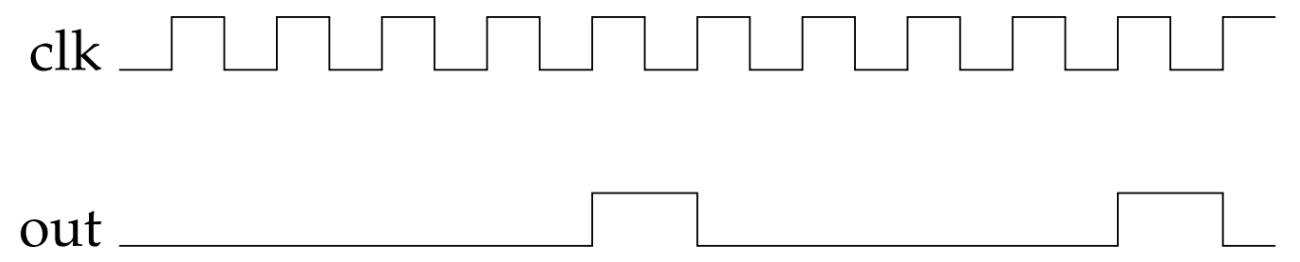
\includegraphics[width=0.78\textwidth]{img/fsm-cinco-ciclos.png}
\end{center}

\vfill
\item Dado o diagrama de estados apresentado abaixo, complete a forma de onda de acordo com o comportamento da m\'{a}quina de estados. Para cada ciclo de clock, indique o estado atual e o valor da sa\'{i}da produzido pela FSM.

\begin{center}
  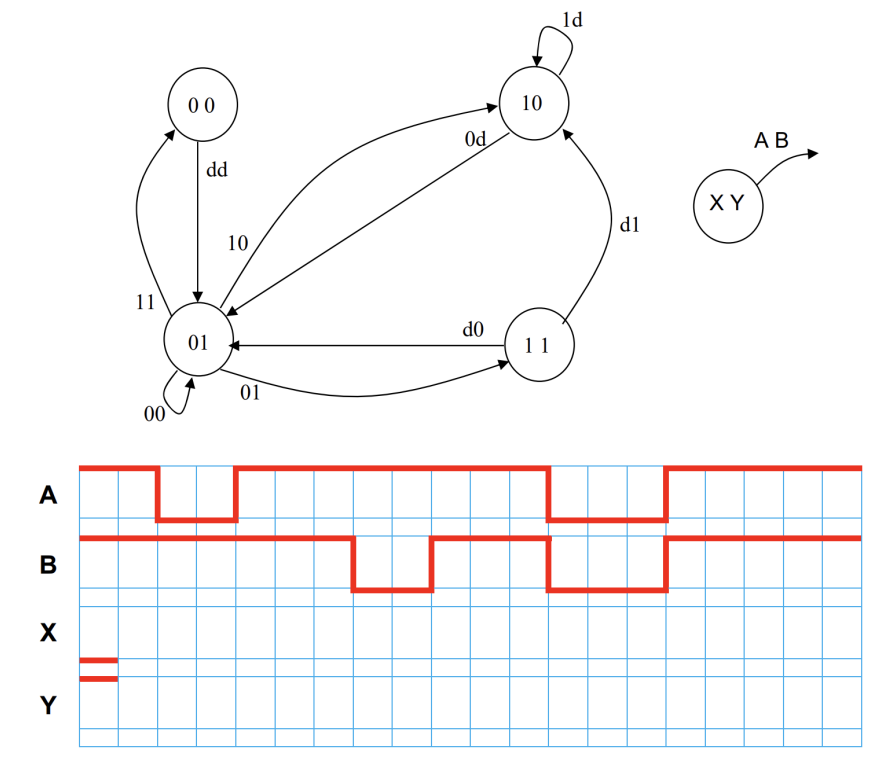
\includegraphics[width=0.48\textwidth]{img/fsm_2.png}
\end{center}

\vfill
\newpage
\vfill
\item Dada a forma de onda apresentada abaixo, complete o diagrama de estados correspondente. Identifique os estados necess\'{a}rios, indique as transi\c{c}\~{o}es entre eles e associe a cada estado o valor de sa\'{i}da produzido pela FSM.

\begin{center}
  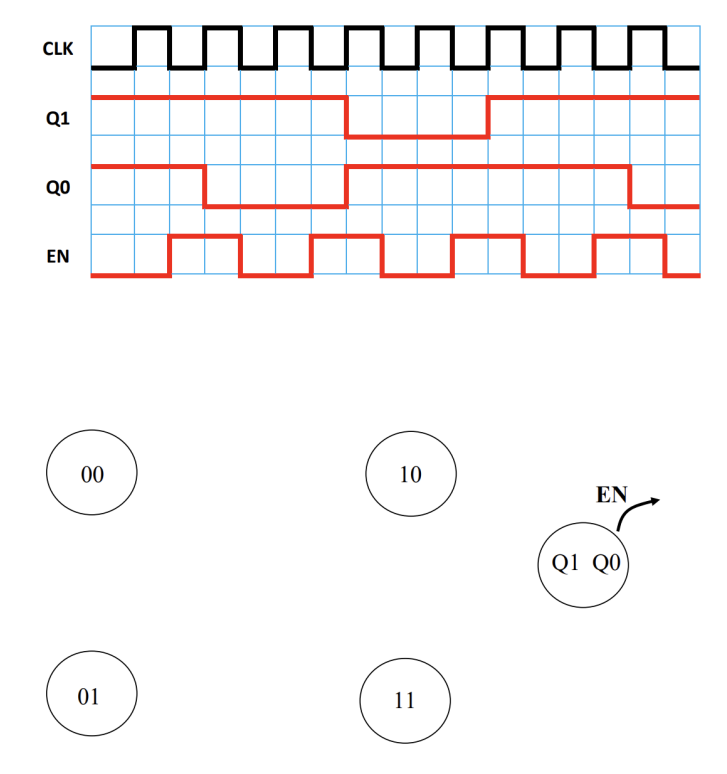
\includegraphics[width=0.48\textwidth]{img/fsm_3.png}
\end{center}

\vfill
\item Dado o diagrama de estados apresentado abaixo, responda:
\begin{enumerate}[label=\alph*)]
  \item Assumindo que a m\'{a}quina de estados est\'{a} inicializada no estado $00$, determine a sequ\^{e}ncia de sa\'{i}da gerada para a sequ\^{e}ncia de entrada:
  \[
    1110\,0011\,1000
  \]
  \item Determine a sequ\^{e}ncia bin\'{a}ria embutida reconhecida por essa m\'{a}quina de estados.
\end{enumerate}

\begin{center}
  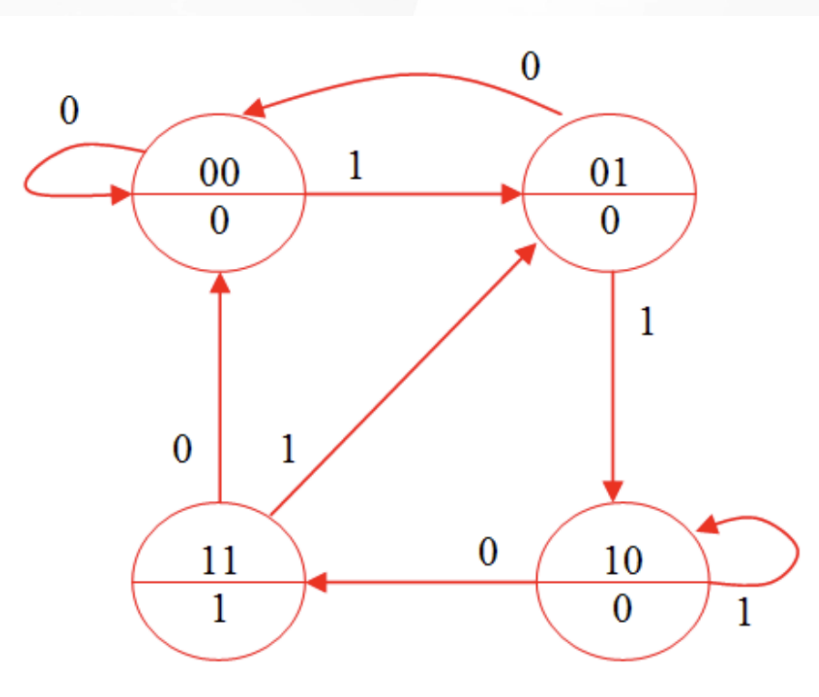
\includegraphics[width=0.48\textwidth]{img/fsm_4.png}
\end{center}

\vfill
\end{enumerate}

\end{document}
